\subsection{他プロジェクトとの差分}
\label{section:project-uniqueness}

\subsubsection{xrdesktop / wxrd}

xrdesktopはLinuxの2Dデスクトップ環境をXR空間から操作することを実現するプロジェクトである
(図\ref{fig:xrdesktop}).Google が主催する OSS 人材育成プロジェクトである
Google Summer of CodeにもOSSプロジェクト側で出るほど信頼度の高いOSSプロジェクトである.
既存の2Dアプリケーションが動作する点はZIGENと同じだが,
アプリケーションがXR空間に3Dのオブジェクトを表示することなどは視野にない.
また,GNOMEやKwinといった既存のデスクトップ環境のウィンドウのミラーを表示するという
実装であるため,ウィンドウのリサイズや移動などを通常の2Dデスクトップ環境と同じように
行うことはできていない.ZIGENが始動した時期と同時期の2021年7月から
同じ開発者が"wxrd"という同様の機能をWaylandコンポジッタを用いて提供するプロジェクトを
試験的に始めており,これはZIGENが2Dアプリケーションを表示している仕組みと近い設計で,
HMDのリフレッシュレートに合わせられていなかった問題などを解消できるとしている
(ZIGENは実現できている).xrdesktop以外にもLinuxに限らず2Dのデスクトップ環境を表示する
機能であれば,商業的にも数多く存在する.しかしいずれにせよ複数の3Dアプリケーションを立ち上げる
環境はない.

\begin{figure}[htbp]
  \begin{minipage}[t]{0.50\linewidth}
    \centering
    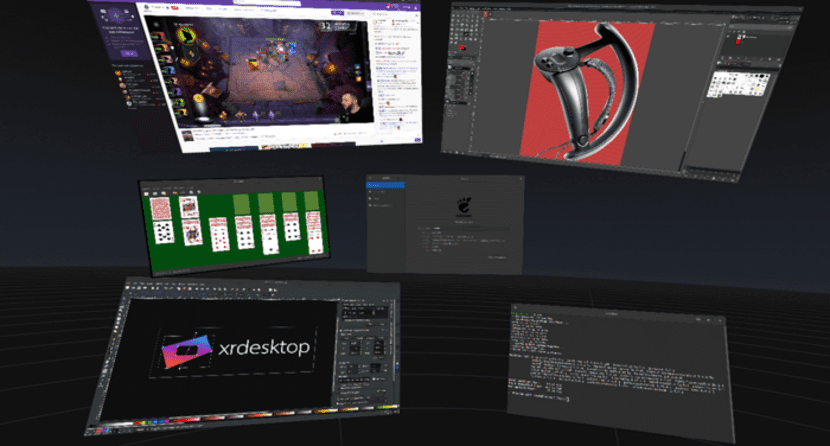
\includegraphics[keepaspectratio, width=\linewidth]{fig/xrdesktop.png}
    \caption{xrdesktop.}
    \label{fig:xrdesktop}
  \end{minipage}
\end{figure}

\subsubsection{OpenXR Overlay}
\label{section:openxr-overlay}

OpenXRとは,ベンダに依存しない統一的なXRプラットフォームやデバイスのインタフェースを提供する
もので,Khronos グループによって策定されており,XRプラットフォーム・デバイス標準化の
デファクトスタンダードになりつつある.
OpenXRの定義の中にはOverlayという仕組みがあり,メインのアプリケーションの上に重ねて
他のアプリケーションを表示できる.またこの合成時にはDepthテストを行うこともできるので,
3Dアプリケーションどうしは前後関係含めて自然に合成して表示できる.

しかしこれは単純にアプリケーションを重ねて表示するだけであり,
複数のアプリケーションがユーザの入力を衝突せずに受け取る仕組みや,
アプリケーション間でのドラッグ \& ドロップのようなベンダに依存しないデータ共有の仕組みは
存在しない.そのため,Overlayのアプリケーションを複数起動して,それらを連携して使うような
使い方には至っていない.

しかしZIGENでは入力の割り振りやデータ共有の仕組みがあるため,マルチアプリケーション・
マルチタスクの環境を提供できる.

\subsubsection{
  Toward General Purpose 3D User Interfaces:
  Extending Windowing Systems to Three Dimensions \cite{forrest}
}
\label{section:forrest}

これはForrestによる2014年の修士論文である.
この論文では,3D没入環境にマルチアプリケーションの環境を提供し,また(当時)XRにおいて
ハードウェアが乱立していてその共通インタフェースがない問題を解決するため,
Windowing Systemを3Dに拡張することを提案し,その場合のウィンドウに相当する概念や,
ハードウェアの抽象化,アプリケーションの描画情報の受け渡し方などについて考察している.

本プロジェクトとの差分としては,実際にユーザが使える状態まで実装される予定がないこと,
ドラッグ \& ドロップなどのデータ共有の仕組みについて言及されていないこと,
その他アプリケーションの描画情報の送り方やアプリケーションの移動などの操作など
細かい部分まで含めると多くあるが,達成したいことはかなり似ており,
Cuboid Windowと呼ばれる概念などはZIGENにも取り入れたりなど,
大変参考にしている論文である.
